\documentclass[11pt]{article}
\usepackage[margin=1in]{geometry}
\usepackage{volfit_preamble}
\graphicspath{{figures/}}

\title{\textbf{Base and Correction}\\[2pt]
\large The Multi-Core Sigmoid: local body detail the wings never feel,
and the budget that keeps it honest\\[2pt]
\normalsize Vol-Fitter Technical Notes, No.~03 --- lecture edition}
\author{Vol-Fitter}
\date{\today}

% Local symbols for this edition (see the notation ledger, Table 1).
\newcommand{\vref}{\sigma_{\mathrm{ref}}}
\newcommand{\Phik}{\Phi_\kappa}
\newcommand{\betP}{\beta_P}
\newcommand{\betC}{\beta_C}

\begin{document}
\maketitle
% Auto-generated by gen_mcs_corrections.py -- do not edit.
\newcommand{\mcscorrmaxerr}{2.55}
\newcommand{\mcscorrbasemaxerr}{153.05}
\newcommand{\mcscorrwingL}{-0.017}
\newcommand{\mcscorrwingR}{0.017}
\newcommand{\mcscorrncores}{2}
\newcommand{\mcscorrnparam}{14}
\newcommand{\mcscorrridge}{0.01}
\newcommand{\mcscorrhinit}{0.40}
\newcommand{\mcscorrkappainit}{5.0}
\newcommand{\mcscorrhlo}{0.15}
\newcommand{\mcscorrhhi}{1.5}
\newcommand{\mcscorrkappalo}{1.0}
\newcommand{\mcscorrkappahi}{12.0}
\newcommand{\mcscorrtargetbeta}{0.055}
\newcommand{\mcscorrtargettailg}{0.250}
\newcommand{\mcscorrtargetgmin}{0.25}
\newcommand{\mcscorrfitgmin}{0.28}
\newcommand{\mcscorrerrRzero}{153.0}
\newcommand{\mcscorrerrRone}{154.7}
\newcommand{\mcscorrerrRtwo}{2.5}
\newcommand{\mcscorrerrRthree}{2.6}
\newcommand{\mcscorrliqinsRthree}{15.0}
\newcommand{\mcscorrliqtrueRzero}{23.9}
\newcommand{\mcscorrliqtrueRthree}{37.7}
\newcommand{\mcscorrarboff}{-2.45}
\newcommand{\mcscorrarbon}{-0.03}
\newcommand{\mcscorrwinggrid}{49}
\newcommand{\mcscorrwingpad}{2}
\newcommand{\mcscorrwingputfactor}{2}
\newcommand{\mcscorrwingbase}{1000}
\newcommand{\mcscorranalyticms}{68.3}
\newcommand{\mcscorrfdms}{161.3}
\newcommand{\mcscorrspeedup}{2.36}
\newcommand{\mcscorrcostdiff}{\ensuremath{1.5\times10^{-15}}}
\newcommand{\mcscorroosbefore}{13.99}
\newcommand{\mcscorroosafter}{13.58}
\newcommand{\mcscorrcostrtwo}{514}
\newcommand{\mcscorrcostrthree}{2023}
\newcommand{\mcscorrputpct}{64}
\newcommand{\mcscorratmpct}{4}
\newcommand{\mcscorrwingminbefore}{-7.9}
\newcommand{\mcscorrwingminafter}{-0.02}
\newcommand{\mcscorrablnoneg}{-30}
\newcommand{\mcscorrablnonerms}{92}
\newcommand{\mcscorrablrepairrms}{25}
\newcommand{\mcscorrablpenaltyrms}{749}
\newcommand{\mcscorrablbothrms}{225}
\newcommand{\mcscorrablflaggedpct}{26}
\newcommand{\mcscorrefanonerms}{75}
\newcommand{\mcscorrefanoneg}{-116}
\newcommand{\mcscorrefarepairrms}{18}
\newcommand{\mcscorrefarepairg}{-12}
\newcommand{\mcscorrefapenaltyrms}{726}
\newcommand{\mcscorrefabothrms}{34}
\newcommand{\mcscorrliqbefore}{10.9}
\newcommand{\mcscorrliqafter}{36.9}
\newcommand{\mcscorrliqflaggedpct}{41}
\newcommand{\mcscorrworstz}{-3.2}
\newcommand{\mcscorrliqflagged}{17 of 30}


\begin{abstract}
Note~02 was about the wings: a smile's tails are a moment reading of the
risk-neutral law, and one convex hyperbola pins them cleanly.  This note fixes
the wings as a solved problem and asks the complementary question --- how to add
detail in the \emph{body} of a smile without disturbing the tails at all.  Some
smiles are not convex: ahead of a binary event, or in bimodally-positioned
names, the curve develops a WW shape (a central trough, a shoulder on each
side).  We prove that no globally convex slice can carry such a shape, so a
hyperbola is structurally disqualified, and we build the answer by
\emph{superposition}: a convex log-cosh \emph{base} owns the wings and the
overall skew, and $R$ signed \emph{corrections} add local humps or notches.  The
mathematical heart is a single fact --- a centred second difference annihilates
affine functions, and the log-cosh primitive is asymptotically affine, so each
correction kernel and its first two derivatives vanish in both tails.  The hats
therefore reshape the body while leaving the base wing slopes \emph{exactly}
fixed: expressiveness and tail control are decoupled by construction.  The
model carries $6+4R$ parameters and a closed-form Durrleman diagnostic, and is
fitted in three layered stages with an analytic Jacobian \mcscorrspeedup$\times$
faster than finite differences.  The second half of the note is the cost of
flexibility.  A flexible model over-fits: on a WW target two cores cut the miss
from \mcscorrbasemaxerr\ to \mcscorrmaxerr\ vol bp, but on a liquid smile a
third core lowers the in-sample error while \emph{raising} the true-curve error
and manufacturing butterfly arbitrage out in the sparse wing.  So the cores
slider is governed --- an identifiability cap, an amplitude ridge, a hard cap at
two, and a default-on put-wing regularizer that is zero on any clean slice.  The
cores slider is a scalpel, not a default.
\end{abstract}

\newpage
\tableofcontents
\newpage

%======================================================================
\section{Two jobs, one curve}
\label{sec:two}

A volatility smile does two jobs, and Note~02 did one of them.  Far from the
money the smile reports the \emph{tails} of the risk-neutral distribution, and
there one convex hyperbola --- raw SVI --- is enough: its two straight wings are
a moment reading, capped by Lee's bound.  Near the money the smile reports the
\emph{body}, the local shape around the forward, and there a hyperbola runs out
of room.  Some smiles are simply not convex.

\begin{proposition}[A convex slice cannot make a WW]
\label{prop:convex}
If total variance $w(k)$ is convex on an interval, it has no interior strict
local maximum there, hence no shoulder flanked by two troughs.  A WW smile ---
a central trough with a shoulder (interior local maximum) on each side --- can
therefore not be represented by any globally convex slice, in particular by raw
SVI, whose $w''>0$ everywhere.
\end{proposition}

\begin{proof}
A convex function on an interval has non-decreasing one-sided derivatives; an
interior strict local maximum would force the derivative to fall from positive
to negative, contradicting monotonicity.  Raw SVI has $w''=b\,s^2/r^3>0$
(Note~02), so it is strictly convex and admits a single minimum only.
\end{proof}

\Cref{fig:whyww} shows the situation.  The convex base misses the two
shoulders by \mcscorrbasemaxerr\ vol bp, and --- the point of the whole note ---
the residual it leaves is \emph{structured}: two localized shoulder features and
a wing compromise, not white noise.  A structured residual invites a structured
correction.  The design question is what that correction should be, and it has a
sharp constraint: it must reshape the body without touching the wings, because
the wings are the solved problem.

\begin{figure}[H]
\centering
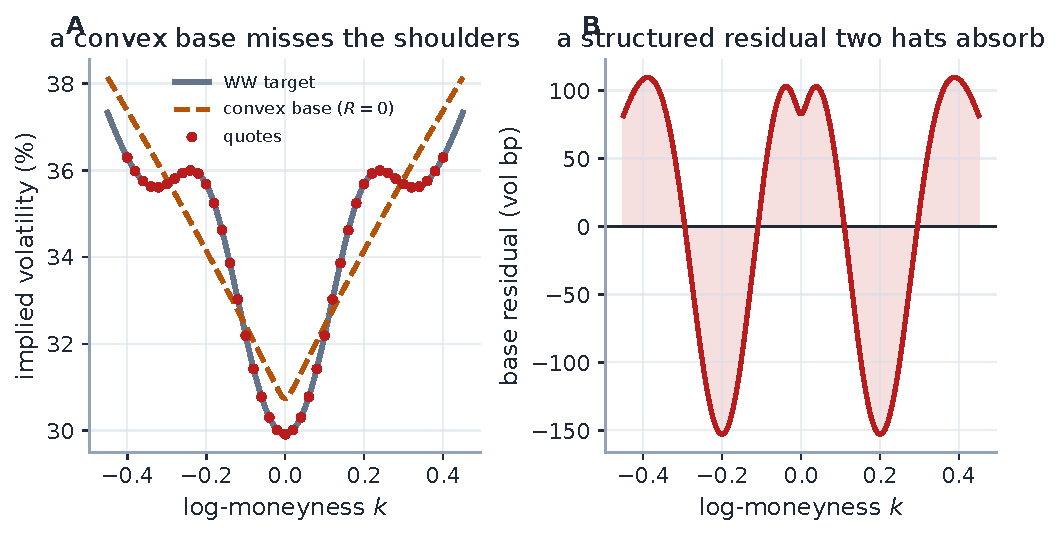
\includegraphics[width=\textwidth]{fig_mcscorr_whyww.pdf}
\caption{Why one convex base is not enough.  Panel A: a WW target (trough plus
two shoulders); the convex base ($R=0$) tracks the overall V but misses both
shoulders by \mcscorrbasemaxerr\ vol bp.  Panel B: the base residual is
structured --- two shoulder features and a wing compromise --- exactly the kind
of thing a few \emph{local} corrections can absorb.}
\label{fig:whyww}
\end{figure}

\paragraph{Conventions and clocks.}
Throughout, $k=\log(K/F)$ is log-moneyness and $v=\sigma_{\mathrm{imp}}^2$ is
\emph{annualized implied variance} --- the quantity this model works in ---
while $w=\tau v$ is total variance.  Here $\tau=\tau_T$ is the production
\emph{variance clock}, calendar time dilated by scheduled events (Notes~00,
11), equal to the calendar year fraction $t$ only when the event clock is off;
production passes $\tau$ to the calibrator, and wherever a bare $t$ plays a time
role below, read $\tau$.  The $z$-scale reference $\vref$ is the \emph{quoted}
volatility nearest the money (with a median-of-quotes fallback when that quote
is degenerate); it is fixed before the fit and never optimized.  A
\emph{volatility basis point} (vol bp) is $10^{-4}$ in volatility.  One
differentiation convention: a prime is the derivative of a one-variable function
($\Phi'$, $B'$, $v'$), a subscripted or explicit $\partial$ is a partial.

\begin{table}[H]
\centering
\small
\setlength{\tabcolsep}{5pt}
\renewcommand{\arraystretch}{1.16}
\begin{tabular}{@{}lll@{}}
\toprule
Symbol & Meaning & First used\\
\midrule
$k,\ z$ & log-moneyness; dimensionless log-strike $k/(\vref\sqrt t)$ & \eqref{eq:zdef}\\
$v(z)$ & annualized implied variance (the modelled quantity) & \eqref{eq:base}\\
$w,\ \tau,\ t$ & total variance $\tau v$; variance clock; calendar fraction & \S\ref{sec:two}\\
$\vref$ & reference vol fixing the $z$-scale & \eqref{eq:zdef}\\
$\Phik$ & log-cosh convexity primitive & \eqref{eq:phi}\\
$V_0,S_0,K_0,z_0$ & base level, slope, convexity, centre (at $z_0$) & \eqref{eq:base}\\
$\kappa_P,\kappa_C$ & asymmetric put/call wing steepnesses & \eqref{eq:base}\\
$B_{c,h,\kappa}$ & zero-wing hat: centre $c$, half-width $h$, steepness $\kappa$ & \eqref{eq:hat}\\
$\alpha_r,\ R$ & signed hat amplitude; number of cores & \eqref{eq:model}\\
$g(k)$ & Durrleman density factor (butterfly diagnostic) & \eqref{eq:g}\\
$\betP,\betC$ & $k$-space total-variance wing slopes & \eqref{eq:betak}\\
\bottomrule
\end{tabular}
\caption{Notation ledger.  Nothing is reused with a second meaning; $v$ is
always variance, $\sigma$ always a volatility.}
\label{tab:ledger}
\end{table}

\begin{invariant}
\begin{enumerate}[leftmargin=1.6em]
\item Adding cores never moves the asymptotic wings: every hat and its first two
derivatives vanish in both tails (\cref{lem:zerowing}), so the base owns the
wing slopes regardless of $R$.
\item Expressiveness is budgeted: cores are capped by the quote count
(\cref{eq:identifiability}) and the surfaced slider is clamped to two.
\item The model reports its own butterfly diagnostic $g$ per fit; it is
\emph{not} arbitrage-free by construction, and the put-wing hinge rows are
exactly zero on any clean slice --- penalty off is byte-identical, penalty on
over a clean slice unchanged to solver tolerance.
\item The parameters are a means, not the object: hats are non-unique by design,
and only the fitted \emph{curve} is contractual (\cref{sec:calib}).
\end{enumerate}
\end{invariant}

\begin{heuristic}
The correction must be \emph{local}: it changes a bounded region of the body but
must not alter the asymptotic wings, which liquid risk-reversals and Lee's law
already pin.  So the kernel must vanish --- in value, slope, \emph{and}
curvature --- in both tails.  ``Zero-wing'' does not uniquely select a kernel (a
Gaussian and its derivatives also vanish), but the centred second difference of
the same log-cosh primitive the base uses is the convenient choice: model and
Jacobian then share one set of analytic jets, the kernel is unit-height at its
centre so its amplitude reads as a variance displacement, and its plateau width
and shoulder steepness are separate dials ($h$, $\kappa$) where a Gaussian has
only one.
\end{heuristic}

%======================================================================
\section{The base owns the wings}
\label{sec:base}

Work in the dimensionless log-strike
\begin{equation}
z=\frac{k}{\vref\sqrt t},
\label{eq:zdef}
\end{equation}
so $z$ measures moneyness in standard deviations and the model is roughly
scale-free across expiries.  The convexity primitive is the \emph{log-cosh}
\begin{equation}
\Phik(u)=\frac{4}{\kappa^2}\log\cosh\!\Big(\frac{\kappa u}{2}\Big),\quad
\Phik'(u)=\frac{2}{\kappa}\tanh\!\Big(\frac{\kappa u}{2}\Big),\quad
\Phik''(u)=\operatorname{sech}^2\!\Big(\frac{\kappa u}{2}\Big).
\label{eq:phi}
\end{equation}
$\Phik$ is a smooth, convex, even softened absolute value.  Two facts about it
carry the whole note.  Near the origin $\Phik(u)\approx u^2/2$ (a rounded
vertex).  Far out it is \emph{asymptotically affine},
\begin{equation}
\Phik(u)=\frac{2}{\kappa}\,|u|-\frac{4}{\kappa^2}\log 2+o(1),
\label{eq:phiaffine}
\end{equation}
a straight wing of slope $2/\kappa$ (\cref{fig:annihilate}A).  For numerical
safety the log-cosh switches to its exact asymptote $|x|-\log2$ beyond $|x|=50$
to avoid $\cosh$ overflow --- clipping $x$ instead would freeze $\Phi$ constant
and destroy the wing slopes.

The base slice and its $z$-derivatives are
\begin{equation}
\begin{aligned}
v_{\mathrm{base}}(z)&=V_0+S_0(z-z_0)+K_0\,\Phi_{\kappa_i}(z-z_0),\\
v_{\mathrm{base}}'(z)&=S_0+K_0\,\Phi_{\kappa_i}'(z-z_0),\qquad
v_{\mathrm{base}}''(z)=K_0\,\Phi_{\kappa_i}''(z-z_0),
\end{aligned}
\label{eq:base}
\end{equation}
with the steepness switching $\kappa_i=\kappa_P$ for $z<z_0$ and $\kappa_C$ for
$z\ge z_0$.  The six parameters are the variance level $V_0$ \emph{at the fitted
centre} $z_0$, the slope $S_0$ there, the convexity amplitude $K_0\ge0$, the
centre $z_0$, and the asymmetric put/call wing steepnesses $\kappa_P,\kappa_C$.
Be precise about what $V_0,S_0$ are \emph{not}: $z_0$ is fitted and generally
$\ne0$, so they are not the ATM level and skew, and the corrections of the next
section can move the full model's ATM handles besides --- the displayed ATM
level, skew and curvature always come from the full curve.  Because $\Phi$ and
$\Phi'$ both vanish at the origin, the slice is $C^2$ across $z_0$ even though
the steepness switches there: the asymmetry is in the \emph{rate} at which each
wing straightens, not a kink.  By \eqref{eq:phiaffine} the asymptotic wing
slopes are
\begin{equation}
v_{\mathrm{base}}'(z)\to S_0\mp\frac{2K_0}{\kappa_{P,C}}\quad(z\to\mp\infty),
\label{eq:wingslopes}
\end{equation}
a left slope $S_0-2K_0/\kappa_P$ and a right slope $S_0+2K_0/\kappa_C$.  These
six numbers set the wings, and --- the design goal --- the corrections must
leave them untouched.

%======================================================================
\section{A basis that vanishes in the tails}
\label{sec:hats}

The correction kernel is the normalized centred second difference of the same
primitive,
\begin{equation}
B_{c,h,\kappa}(z)=\frac{\Phik(u-h)-2\Phik(u)+\Phik(u+h)}{2\Phik(h)},
\qquad u=z-c,
\label{eq:hat}
\end{equation}
centred at $c$, of half-width $h$ and steepness $\kappa$, normalized so
$B_{c,h,\kappa}(c)=1$.  Its derivatives are the same second difference of $\Phi'$
and $\Phi''$ over the same normalizer.  Now the one fact everything rests on.

\begin{lemma}[Zero wings]
\label{lem:zerowing}
$B_{c,h,\kappa}(z)\to0$, $B_{c,h,\kappa}'(z)\to0$ and
$B_{c,h,\kappa}''(z)\to0$ as $z\to\pm\infty$.
\end{lemma}

\begin{proof}
A centred second difference annihilates affine functions: for any $L(u)=pu+q$,
$L(u-h)-2L(u)+L(u+h)=0$ identically.  By \eqref{eq:phiaffine} $\Phi$ is affine
plus $o(1)$ in each tail, so its second difference tends to $0$ there.  The same
argument applies to $\Phi'$ (which tends to the constants $\pm2/\kappa$, affine
of zero slope) and to $\Phi''$ (which decays), so $B$, $B'$ and $B''$ all vanish
in both tails.
\end{proof}

\Cref{lem:zerowing} is the whole design.  Adding $\alpha B$ to the base changes
the body but leaves the wing slopes \eqref{eq:wingslopes} \emph{exactly}
unchanged.  The amplitude $\alpha$ is in variance units and, since $B(c)=1$, is
approximately the variance displacement at the centre; a positive $\alpha$
raises a shoulder, a negative one digs a notch.  The centre curvature
$B''(c)=(\operatorname{sech}^2(\kappa h/2)-1)/\Phik(h)<0$, so a positive hat is
locally concave (a hump), as a shoulder should be.  \Cref{fig:annihilate}
draws both halves of the mechanism.

\begin{figure}[H]
\centering
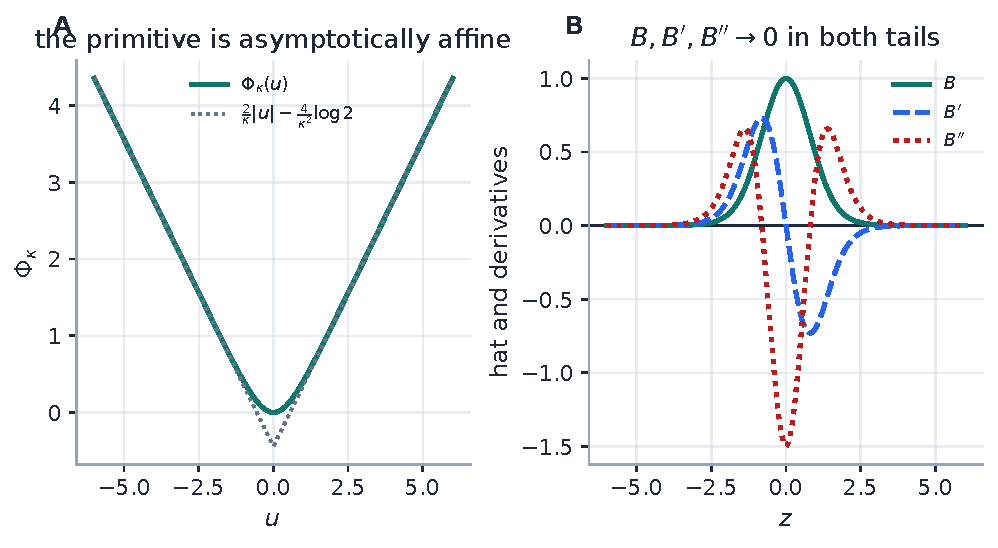
\includegraphics[width=\textwidth]{fig_mcscorr_annihilate.pdf}
\caption{The mechanism, in two facts.  Panel A: the log-cosh primitive is
asymptotically affine --- it merges with the straight line $\frac2\kappa|u|
-\frac4{\kappa^2}\log2$ in both tails, differing only at the rounded vertex.
Panel B: the centred second difference of an asymptotically-affine function is a
localized bump whose value, slope \emph{and} curvature all decay to zero.  A
correction built this way is silent in the wings to all three orders.}
\label{fig:annihilate}
\end{figure}

\paragraph{Exercise 1.}
Verify the annihilation directly: for $L(u)=pu+q$, expand
$L(u-h)-2L(u)+L(u+h)$ and confirm it is identically zero.  Conclude that
\emph{any} asymptotically-affine primitive --- not just the log-cosh --- yields
a zero-wing kernel by the same second difference, and that the log-cosh is a
convenience (shared jets, unit height, two dials), not a necessity.

%======================================================================
\section{The full model: superposition}
\label{sec:model}

The Multi-Core Sigmoid (MCS) slice is the base plus $R$ signed corrections,
\begin{equation}
\boxed{\;v_R(z)=v_{\mathrm{base}}(z)+\sum_{r=1}^{R}\alpha_r\,B_{c_r,h_r,\kappa_r}(z),\;}
\qquad w(k)=t\,v_R(z),
\label{eq:model}
\end{equation}
with $6+4R$ parameters.  \Cref{fig:superpose} shows the decomposition on the WW
fit: the convex base owns the V, and two signed hats add precisely the two
shoulders, each localized.  By \cref{lem:zerowing} every member of this family
has the \emph{same asymptotic wings as its base}, whatever $R$ is ---
\cref{fig:wingneutral} makes that visible, overlaying the base and the
base-plus-hats: the bodies differ, the wings coincide, and the difference
$\sum_r\alpha_r B_r$ decays to zero out of the money.  Expressiveness in the
body and control of the tails are, by construction, two separate concerns.

\begin{figure}[H]
\centering
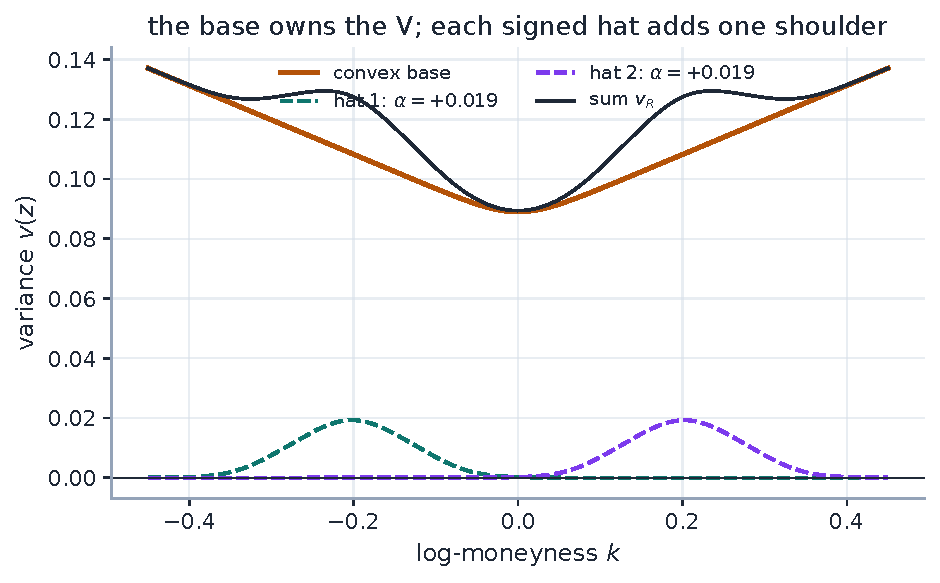
\includegraphics[width=0.92\textwidth]{fig_mcscorr_superpose.pdf}
\caption{Superposition.  The convex base carries the overall V; each signed hat
is a localized bump that adds one shoulder; their sum is the fitted slice.  The
hats live where the residual of \cref{fig:whyww}B lived.}
\label{fig:superpose}
\end{figure}

\begin{figure}[H]
\centering
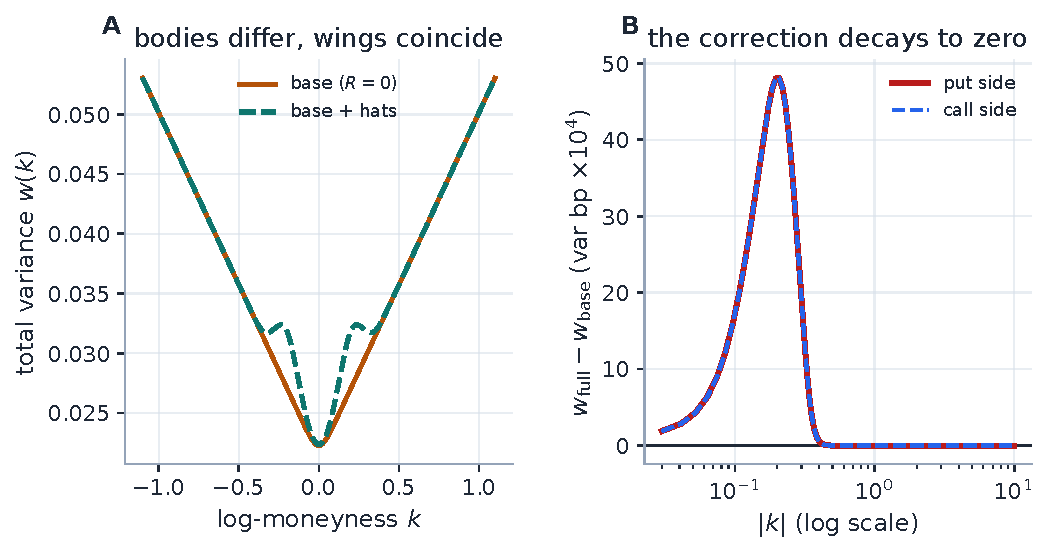
\includegraphics[width=\textwidth]{fig_mcscorr_wingneutral.pdf}
\caption{The correction is local.  Panel A: base and base-plus-hats differ in
the body but their total-variance wings coincide exactly.  Panel B: the
difference $w_{\mathrm{full}}-w_{\mathrm{base}}$ is a bump that decays to zero in
both tails (the put and call sides overlie), so the wing slopes are preserved
pointwise, not merely on average.}
\label{fig:wingneutral}
\end{figure}

There is one honest subtlety, and it is worth stating in Note~02's vocabulary.
\emph{Wing-neutral} is weaker than \emph{Lee-compatible}.  The hats preserve the
base wing slopes, but nothing constrains those base slopes to be admissible in
the first place.  In total-variance $k$-space the wing slopes are
\begin{equation}
\betP=\frac{\sqrt{\tau}}{\vref}\Big(\frac{2K_0}{\kappa_P}-S_0\Big),\qquad
\betC=\frac{\sqrt{\tau}}{\vref}\Big(S_0+\frac{2K_0}{\kappa_C}\Big),
\label{eq:betak}
\end{equation}
and admissibility asks $0\le\betP,\betC\le2$ (upward wings under Lee's cap).
The calibration bounds of \cref{sec:calib} do \emph{not} enforce this: the hats
guarantee the base slopes are \emph{preserved}, and whether the preserved slopes
are themselves Lee-clean is a separate, diagnosed condition (the cross-model
wing treatment is Note~09).

The cores count $R$ is the user's ``cores'' slider --- the direct analogue of
the LQD Legendre order, the one dial that trades expressiveness for parsimony.
The rest of the note is about reading that dial correctly.

%======================================================================
\section{Static no-arbitrage}
\label{sec:noarb}

Butterfly-freedom is the Durrleman condition, evaluated by converting the
$z$-space variance and its derivatives to total-variance $k$-space via
$k=\vref\sqrt t\,z$ and $w=tv$:
\begin{equation}
g(k)=\Big(1-\frac{k\,w'}{2w}\Big)^2-\frac{w'^2}{4}\Big(\frac1w+\frac14\Big)+\frac{w''}{2}\ \ge\ 0.
\label{eq:g}
\end{equation}
Unlike LQD, and unlike the base alone, \emph{MCS is not arbitrage-free by
construction}.  A signed hat can drive the raw variance negative (there is no
positivity penalty in the fit) or, more commonly, break convexity locally, so
the equivalence ``$g\ge0\iff$ non-negative density'' comes with conditions worth
stating: it presumes $v_R>0$, a smooth slice, and appropriate wings, and on a
finite grid $g$ is a \emph{diagnostic}, never a global certificate.

\begin{remark}[Which curve's $g$?]
Positivity and the floor interact in code.  Pricing floors the variance at
$10^{-8}$, and the reported diagnostic is the Durrleman functional of that
\emph{priced} (floored) curve: where the floor binds, the priced slice is
locally constant, its derivatives are zero, and the separate raw-positivity
check flags the slice as not butterfly-free.  (An earlier revision mixed the
floored \emph{value} with the raw \emph{derivatives} --- a functional of no
curve at all; fixed and test-locked.)  The \emph{penalty}-path $g$ inside the
calibrator deliberately keeps the raw derivatives instead: at a collapsed-variance
grid point the $1/w$ term then explodes negative, a harsh de-facto barrier
against hats that drive variance through zero.
\end{remark}

\subsection{Where the arbitrage lives, and the put-wing regularizer}
\label{sec:wingpen}

When cores over-reach they break \eqref{eq:g} not near the money --- where dense
quotes discipline the curvature --- but out in the sparsely quoted wings, where
each hat's local curvature is unconstrained by data.  The offline backtest
localizes the violation sharply: across the audited over-parametrized
spike-regime refits, about \mcscorrputpct\% of the $g<0$ points sit in the
\emph{put} wing (the steep, variance-loaded side of the equity skew) against
only $\sim\mcscorratmpct\%$ near the money, with the worst point at a median
standardized moneyness $z\approx\mcscorrworstz$.  To discipline that region the
joint refine carries an optional \emph{put-wing Durrleman penalty}: on a grid
$\{z_j\}$ of $M=\mcscorrwinggrid$ points spanning the quoted range extended
$\Delta z=\mcscorrwingpad$ into both tails, it appends the rows
\begin{equation}
r^{\mathrm{wing}}_j=\sqrt{\lambda_j}\,\max\!\big(-g(z_j),\,0\big),
\qquad \lambda_j=\Lambda\,\lambda_0\,\big(1+\1\{z_j<0\}\big),
\label{eq:wingpen}
\end{equation}
with base strength $\lambda_0=\mcscorrwingbase$, surfaced dial
$\Lambda=\texttt{sivWingPenaltyPct}/100$ (product default $1$; $0$ disables),
and the indicator \emph{doubling} the weight on the put side to match the
measured asymmetry.  Because $\max(-g,0)=0$ wherever the slice is
butterfly-free, \eqref{eq:wingpen} is exactly zero on an admissible fit: a
liquid, arbitrage-free name is byte-identical with or without it.  The penalty
bites only where a hat would otherwise manufacture a wing violation.

\Cref{fig:wingarb} demonstrates the penalty on a genuine over-reach.  A convex
truth is handed two arbitraged put-wing quotes (a localized non-convex kink of
the kind a per-strike de-Americanization can produce, Note~05); a hat chases the
kink and drives $g$ to \mcscorrarboff\ in the put wing.  The same quotes refit
with the penalty on are pulled back to the admissible boundary
($g\ge\mcscorrarbon$) --- at the cost of fitting the arbitraged quotes less,
which is the right trade.

\begin{figure}[H]
\centering
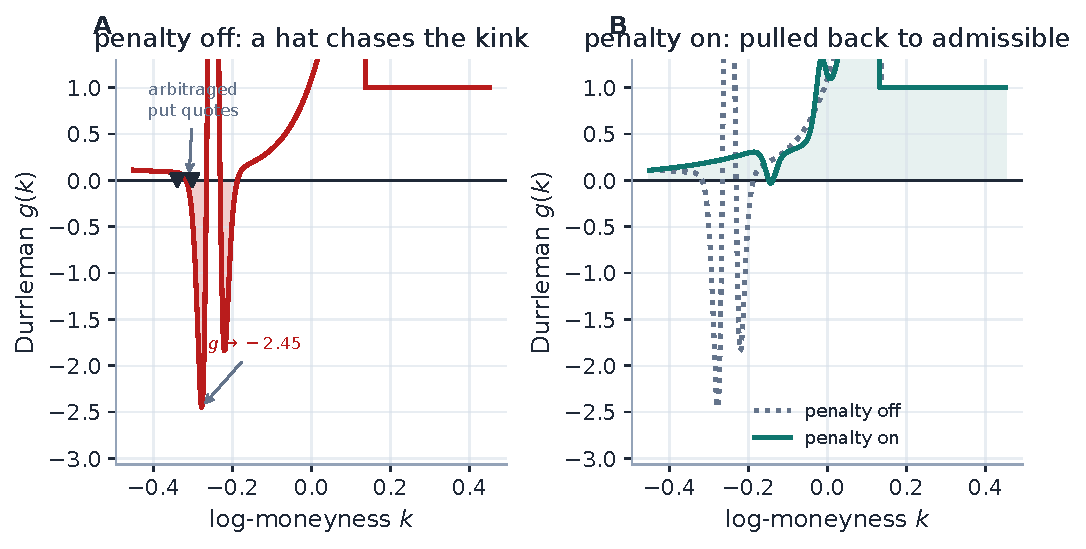
\includegraphics[width=\textwidth]{fig_mcscorr_wingarb.pdf}
\caption{The put-wing penalty.  Panel A: with the penalty off, a hat chases two
arbitraged put quotes and breaks convexity, $g\to\mcscorrarboff$ in the put wing
(the positive spike is the local hump the kink induces; the $y$-axis is clipped
to the violation).  Panel B: with the penalty on, the fit is pulled back to
$g\ge\mcscorrarbon$ there, fitting the bad quotes less.  The hinge is one-sided
and zero wherever $g\ge0$.}
\label{fig:wingarb}
\end{figure}

\begin{heuristic}
The penalty is a one-sided hinge on the same $g$ the model already reports.
Although its grid covers the quoted region too, it \emph{bites} only where the
model extrapolates: where quotes are dense they discipline the curvature, so
$g\ge0$ there and the rows are zero.  It does not \emph{guarantee} $g\ge0$ (a
soft penalty trades the violation against the data fit), but on genuinely
arbitraged illiquid wings it shrinks the worst violation by orders of
magnitude --- the backtest measured a median wing $\min g$ moving from
$\approx\mcscorrwingminbefore$ to $\approx\mcscorrwingminafter$.
\end{heuristic}

Beyond the core diagnostic and this penalty, two further layers stand at
increasing distance from the fit: an always-on advisory that measures the
remaining extrapolated-region $g<0$ per fit, and an export-only wing projection
that raises exported prices to convexity while leaving the fitted core pinned
(Note~09).  None of them turns a fitted MCS slice into a certified
butterfly-free object; together they bound, measure, and clean at the boundary.

%======================================================================
\section{Calibration}
\label{sec:calib}

The fit is a three-stage workflow that respects the model's layered structure.
\begin{enumerate}[leftmargin=1.6em]
\item \textbf{Base fit ($R=0$).}  Fit the six base parameters to the mid quotes
under bound constraints, from a data-driven start that reads the ATM variance,
the local skew and the local convexity off three interpolated points.  This
stage is always mid, so its residual is meaningful for the next.
\item \textbf{Greedy hat seeding.}  Compute the base residual in variance space
and place each hat at the largest remaining $|\text{residual}|$, masking a
neighbourhood after each placement so two hats cannot seed on one feature.  Each
seed starts at half-width $h=\mcscorrhinit$ and steepness $\kappa=\mcscorrkappainit$,
its amplitude read from the local residual and clipped to $[-1,1]$.
\item \textbf{Joint bounded refine.}  Refine all $6+4R$ parameters together
under the requested objective (mid or band) with a mild ridge
$\sqrt{\varrho}\,\alpha_r$ on the hat amplitudes, $\varrho=\mcscorrridge$.  The
ridge keeps overlapping cores from exploding against each other without biasing
a well-determined amplitude.
\end{enumerate}
All positive parameters ($K_0$, the steepnesses, the hat half-widths and
steepnesses) are bound-constrained directly through scipy's trust-region
reflective solver, the hat half-width held in $[\mcscorrhlo,\mcscorrhhi]$ and
its steepness in $[\mcscorrkappalo,\mcscorrkappahi]$.

\paragraph{The identifiability cap.}
The cores count is capped by the quote count,
\begin{equation}
R\le\Big\lfloor\frac{N_{\mathrm{quotes}}-6}{4}\Big\rfloor,
\label{eq:identifiability}
\end{equation}
so the model never has more free parameters than quotes, guarding sparse
short-dated chains against spurious narrow kernels.  Be precise about what this
does and does not prevent: it caps only the \emph{hats}, so with
$N_{\mathrm{quotes}}\ge6$ it stops under-identified hats --- but the
application's minimum of five included quotes per node means the six-parameter
base can still be fitted to five quotes (one parameter over the data; the bounds
and the data-driven start keep it tame, but it is not a guarantee).

\paragraph{The hard cap, and non-unique hats.}
Independently of \eqref{eq:identifiability}, the surfaced slider is
\emph{hard-capped at two}, $R\in\{0,1,2\}$: \cref{sec:capacity} shows a third
core buys almost nothing out-of-sample while manufacturing wing arbitrage, so
any incoming setting above two is silently clamped.  Precision matters: the
clamp lives in the \emph{schema}, not the calibrator --- the library
\texttt{calibrate\_sigmoid(n\_cores=3)} runs happily and its tests exercise it.
The cap is a product decision at the settings boundary; research code below it
keeps the full family.  Relatedly, the hats are \emph{non-unique} by
construction: two overlapping hats can trade amplitude against each other, so
the round-trip test recovers the \emph{curve}, not the parameters, and nothing
downstream ever consumes a hat parameter.  The individual
$(\alpha_r,c_r,h_r,\kappa_r)$ are not trader handles.

The refine stage carries the same optional blocks as the other models --- band
fit (Note~07), var-swap target (Note~08), the model-agnostic calendar hinge
(Note~10), prior persistence (Note~13), the put-wing regularizer
\eqref{eq:wingpen}, and the default-off tapered extrapolated-region fences
(Notes~09--10) --- each byte-identical to its own absence, so the sigmoid
overlay is no longer a prior exception.

\begin{perfbox}
The dominant cost of an $R$-core fit is the $(6+4R+1)$-evaluation
finite-difference Jacobian.  The closed-form Jacobian of the residual stack
(data $+$ ridge $+$ calendar), propagated through the log-cosh primitive,
replaces it in one pass: a fresh run measured \mcscorrfdms\,ms $\to$
\mcscorranalyticms\,ms (\mcscorrspeedup$\times$), optimum unchanged to
\mcscorrcostdiff\ in cost.  Scope of that number --- it is the $R=2$ mid
\emph{final-refine} microbenchmark alone (base fit, seeding and the
product-default wing penalty excluded), single-threaded, not an end-to-end
calibration timing.  The analytic path is gated to the var-swap/prior-free
configuration.  When the wing penalty \eqref{eq:wingpen} or the extrapolation
fences are active the Jacobian is \emph{hybrid}: analytic for the
data/ridge/calendar rows and finite-difference only for the small penalty
blocks, so the penalized fit keeps most of the analytic speed.  See
\cref{app:perf}.
\end{perfbox}

\begin{figure}[H]
\centering
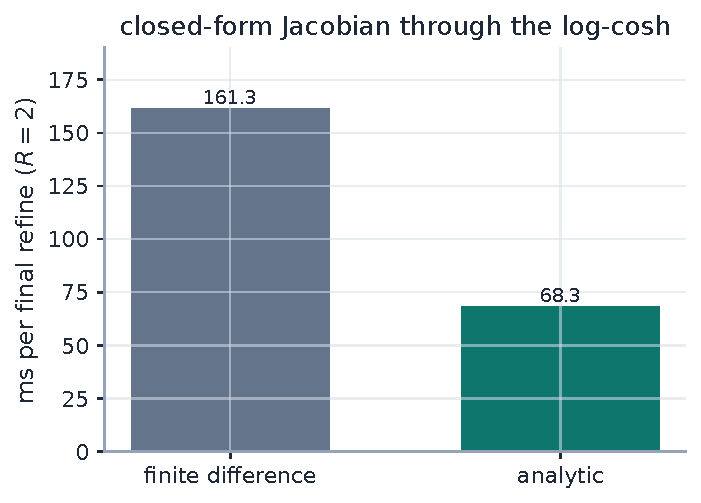
\includegraphics[width=0.56\textwidth]{fig_mcscorr_timing.pdf}
\caption{The closed-form Jacobian through the log-cosh replaces the
$(6{+}4R{+}1)$-evaluation finite difference on the $R=2$ final refine
(\mcscorrspeedup$\times$ here; machine-dependent, protocol in \cref{app:perf}).}
\label{fig:timing}
\end{figure}

\paragraph{Exercise 2.}
The centre curvature is $B''(c)=(\operatorname{sech}^2(\kappa h/2)-1)/\Phik(h)$.
Show it is strictly negative for every $h,\kappa>0$, and deduce that a positive
amplitude always produces a local hump and a negative amplitude a local notch ---
so the \emph{sign} of $\alpha_r$ is the only thing a reader needs to know a
core's qualitative effect.

%======================================================================
\section{Expressiveness on a budget}
\label{sec:capacity}

A flexible model has two failure modes, and MCS shows both cleanly.  Too few
cores and it \emph{underfits}: on the WW target one convex base leaves a
\mcscorrerrRzero\ vol bp miss, and --- because a single off-centre hat cannot
address two symmetric shoulders --- one core barely helps
(\mcscorrerrRone\ bp); only at $R=2$ does the error collapse, to
\mcscorrerrRtwo\ bp (\cref{fig:capacity}A).  Too many cores and it
\emph{over-fits}: on a liquid, genuinely convex smile fitted to noisy quotes,
each extra core drives the in-sample error down but the error against the
\emph{true} curve up --- from \mcscorrliqtrueRzero\ vol bp at $R=0$ to
\mcscorrliqtrueRthree\ bp at $R=3$, the classic bias--variance scissor
(\cref{fig:capacity}B).  The cores are chasing quote noise.

\begin{figure}[H]
\centering
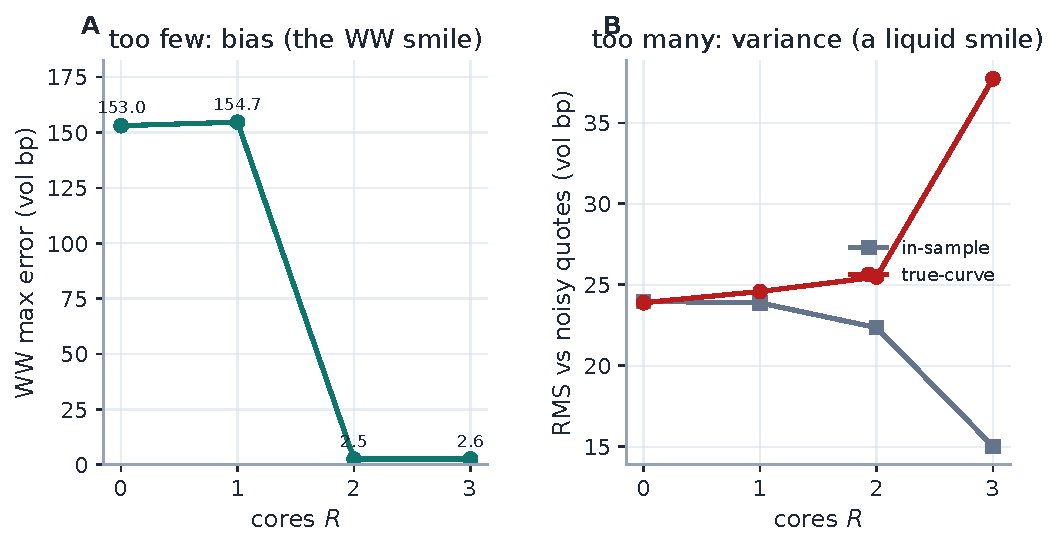
\includegraphics[width=\textwidth]{fig_mcscorr_capacity.pdf}
\caption{The two failure modes of the wrong core count.  Panel A (a WW smile):
too few cores is bias --- the error stays near \mcscorrerrRzero\ vol bp until
two hats can seat both shoulders, then collapses; a third buys nothing.  Panel B
(a noisy liquid smile): too many cores is variance --- the in-sample error keeps
falling while the true-curve error rises, the signature of over-fitting.  The
right core count is neither the most nor the fewest.}
\label{fig:capacity}
\end{figure}

This is why the slider is governed rather than free.  The backtest made the cost
concrete on real data: on liquid index chains the extra cores chase quote noise
and manufacture butterfly arbitrage (the analytic diagnostic flags $g<0$ on a
majority of nodes at $R\ge2$ on dense data), while the base $R=0$ behaves
comparably to SVI.  The honest marginal number for the third core, from the
spike replay: out-of-sample RMS \mcscorroosbefore$\to$\mcscorroosafter\ bp --- a
$0.41$ bp gain --- for roughly four times the fit cost
($\mcscorrcostrtwo\to\mcscorrcostrthree$\,ms in that harness) and worse arbitrage.
Not negative precision, but nowhere near worth it.  Hence the hard cap at two,
on top of the identifiability cap, the amplitude ridge, and the $g$ diagnostic.

\begin{caution}
With great expressiveness comes over-fitting, and MCS is the one model in the
series where the default posture is restraint.  The operational guidance:
\emph{use cores only when the smile is genuinely non-convex} (events, bimodal
positioning), and prefer LQD or Local-Vol for routine fitting.  The cores slider
is a scalpel, not a default --- which is why the product default model is LQD,
and MCS is the event/WW specialist.
\end{caution}

\begin{example}[title={Case file: two defences, one pathology}]
The put-wing violation has \emph{two} sources: the flexible model genuinely
over-reaching (cured by the penalty \eqref{eq:wingpen}), and \emph{arbitraged
inputs} --- the per-strike de-Americanization of Note~05 can hand every model a
call curve already slightly non-convex in the wings.  An ablation isolating the
two defences (the de-Am convex repair of Note~05 versus the penalty) on illiquid
American ETFs found them \emph{complementary, not redundant}.  On the arb-prone
population (medians over 38 nodes): with neither, worst $g\approx\mcscorrablnoneg$
and in-sample RMS \mcscorrablnonerms\ bp; the de-Am repair alone cuts the
violation about threefold \emph{and lowers} the RMS to \mcscorrablrepairrms\ bp
(it removes the arbitraged quotes the model was chasing); the penalty alone
nearly eliminates the violation but at \mcscorrablpenaltyrms\ bp (it must fight
those same quotes); both attain the penalty's arbitrage reduction at
\mcscorrablbothrms\ bp, because the inputs are cleaned before the constraint is
imposed.  Reduction, not elimination: even with both defences on,
\mcscorrablflaggedpct\% of the population stays flagged.  One node makes it
vivid (EFA in the Aug-2024 spike, 11 days, 22 quotes): neither,
\mcscorrefanonerms\ bp with worst $g=\mcscorrefanoneg$; repair alone, a tight
\mcscorrefarepairrms\ bp but $g=\mcscorrefarepairg$; penalty alone,
arbitrage-free but \mcscorrefapenaltyrms\ bp; both, arbitrage-free at
\mcscorrefabothrms\ bp.  \emph{The fence is expensive only when it must fight
arbitraged inputs --- cleaning the inputs at the source is what makes the
constraint affordable.}
\end{example}

%======================================================================
\section{Worked example: a WW smile}
\label{sec:example}

The target in \cref{fig:whyww} is a synthetic WW built to be \emph{globally}
admissible, not merely clean on a window.  Its total variance is a hyperbolic
base plus two Gaussian shoulders,
$w(k)=a+b\sqrt{k^2+\varsigma^2}+\sum_\pm A\,e^{-((k\mp c)/s)^2}$.  Gaussians
vanish with all derivatives, so the $w$-wings are exactly linear with slope
$\beta=\mcscorrtargetbeta\le2$ (Lee-admissible for every $k$), and $g$ tends to
the positive limit $(4-\beta^2)/16=\mcscorrtargettailg$ in both tails.  The
generator computes $g$ from analytic jets (no finite differences, the
measurement lesson of Note~02) and asserts $g>0$ for target \emph{and} fit on a
dense grid to $|k|=12$ before writing anything.

The base ($R=0$) fits it only to \mcscorrbasemaxerr\ vol bp, missing both
shoulders.  Two hats ($R=2$, $6+4\cdot2=\mcscorrnparam$ parameters) reduce the
maximum error to \mcscorrmaxerr\ vol bp --- report two numbers and keep them
separate: the \emph{quote} error \mcscorrmaxerr\ vol bp is the fit's miss on the
target, while the fit stays globally butterfly-clean, its wide-grid minimum
$g=\mcscorrfitgmin$ (the target's is \mcscorrtargetgmin).  Meanwhile the
preserved base wing slopes $(S_0-2K_0/\kappa_P,\,S_0+2K_0/\kappa_C)=
(\mcscorrwingL,\,\mcscorrwingR)$ in $z$-space are exactly the base's, cores or
no cores.  \Cref{fig:gclean} plots the diagnostic for both curves.

\begin{figure}[H]
\centering
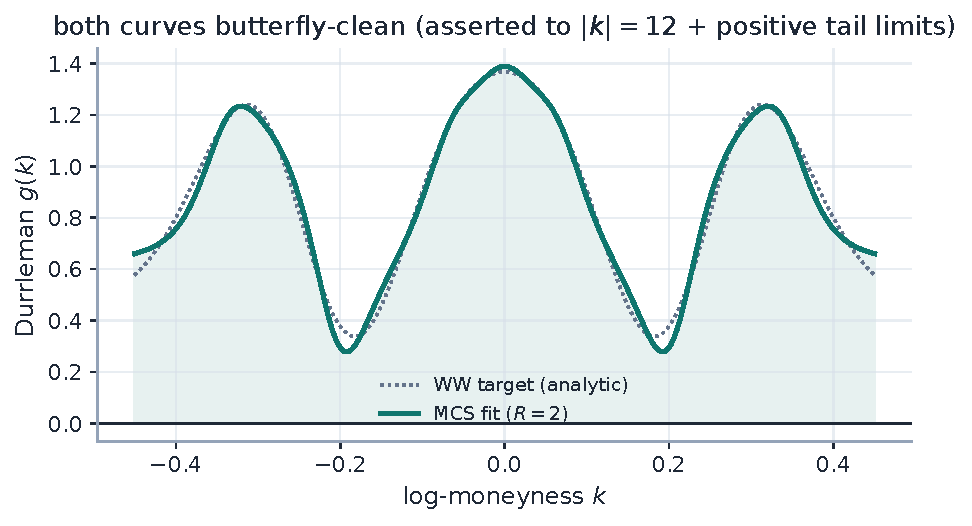
\includegraphics[width=0.86\textwidth]{fig_mcscorr_gclean.pdf}
\caption{The butterfly diagnostic for the fitted slice and the target it chased.
Both stay non-negative on the display window; with the wide-grid assertion to
$|k|=12$ and the positive analytic tail limits, the cleanliness claim is global,
not per-window.}
\label{fig:gclean}
\end{figure}

\begin{remark}[The target must be clean too --- a bug fixed twice]
\label{rem:targetbug}
A diagnostic is only as strong as the exercise it certifies, and this figure's
target needed two rounds of honesty.  An early revision built a WW target whose
\emph{own} Durrleman function dipped to $g\approx-0.38$ near the shoulders: the
synthetic ``market'' itself carried butterfly arbitrage, so no admissible slice
could both track it and honour $g\ge0$, and the figure's claim was quietly
false.  The first fix re-chose the shoulder amplitudes and widths (the
shoulder-top curvature scales like $2A/s^2$, which drives $w''$, hence $g$,
negative) --- but that target was built in \emph{volatility} space with linear
tails, so its total variance grew quadratically and still violated Lee far
outside the window: cleanliness only per-window.  The current construction
builds the target in \emph{total-variance} space, so the $w$-wings are exactly
linear and the tail $g$ limit is positive analytically.  The lesson is the same
one Note~02 drew about measuring $g$: compute it from analytic jets, and certify
globally (a wide grid plus a tail limit), never on a plotted window alone.
\end{remark}

\paragraph{Exercise 3.}
The identifiability cap \eqref{eq:identifiability} counts parameters against
quotes.  Show that with $N_{\mathrm{quotes}}=5$ it gives $R=0$, yet the base
alone has six parameters --- one more than the data.  Explain why this is not an
outright failure (bounds and the data-driven start regularize it) but is also
not an identifiability guarantee, and why a desk should distrust the individual
base parameters, though not necessarily the fitted curve, on such a chain.

%======================================================================
\section{What is original, and limitations}
\label{sec:original}

The genuinely original elements are the \emph{zero-wing hat}
(\eqref{eq:hat}--\cref{lem:zerowing}) --- a correction basis local in the body
and provably neutral in the wings, so expressiveness and tail control are
decoupled by an elementary annihilation property --- and the \emph{layered
three-stage calibration} that places the corrections on residuals rather than
optimizing them blind.  Together they let one model span from a clean index
smile ($R=0$, a convex family in its own right, not an SVI equivalent) to an
event-shaped WW smile ($R=2$) on a single slider.  (A WW \emph{implied-volatility}
curve suggests, but does not by itself prove, a bimodal risk-neutral density:
the density is the Breeden--Litzenberger second derivative of price, not a
re-reading of the vol curve.)

Limitations, stated plainly.  MCS is \emph{not} arbitrage-free by construction:
signed hats can drive variance negative or break convexity, so $g$ is a reported
diagnostic and the wing penalty a soft, non-guaranteeing fence
(\cref{sec:noarb}).  Its wings are wing-\emph{neutral}, not Lee-guaranteed:
admissibility of the preserved base slopes is a separate check
\eqref{eq:betak}.  It over-fits liquid data when the slider is pushed, which is
why the surfaced cap is two and the default model is LQD.  And its hats are
non-unique, so comparisons across fits must be made on curves and handles, never
on the correction parameters.  The cores slider earns its keep exactly when the
smile is genuinely non-convex, and nowhere else.

\appendix
%======================================================================
\section{Hyperparameter atlas}
\label{app:atlas}

\begin{longtable}{p{0.25\textwidth}p{0.13\textwidth}p{0.54\textwidth}}
\caption{Multi-Core Sigmoid (MCS) hyperparameters.}\label{tab:atlas}\\
\toprule Knob & Default & Role\\ \midrule
\endfirsthead
\toprule Knob & Default & Role\\ \midrule
\endhead
\multicolumn{3}{@{}p{0.94\textwidth}@{}}{\emph{Surfaced.  Product defaults shown
(the product's default model is LQD; these apply when MCS is selected).  Library
defaults differ: $R=0$, penalty off.}}\\ \midrule
\texttt{nCores} $R$ & $2$ & Number of zero-wing hats, $R\in\{0,1,2\}$
(schema-clamped at two on every parse; the library is uncapped, and
\eqref{eq:identifiability} may reduce $R$ further).  $0$ = pure base.\\
\texttt{sivWingPenaltyPct} $\Lambda$ & $100$ & Put-wing Durrleman penalty
\eqref{eq:wingpen} strength; $100=$ base $\lambda_0=\mcscorrwingbase$, $0=$ off.\\
\texttt{sigmoidRidge} $\varrho$ & \mcscorrridge & $\ell^2$ penalty on hat
amplitudes in the refine stage.\\
\texttt{midAnchorWeight} & $0.05$ & Band-fit mid anchor (Note~07).\\
\texttt{weightScheme} & \texttt{equal} & Per-quote weights (Note~07).\\
\texttt{calendarWeight} & $10^{6}$ & Calendar hinge penalty (Note~10).\\
\texttt{extrapEnforce} & off & Tapered extrapolated-region fences (Notes
09--10); hybrid Jacobian when on.\\
\midrule
\multicolumn{3}{l}{\emph{Internal (seeding / bounds)}}\\ \midrule
\texttt{\_H\_INIT} & \mcscorrhinit & Hat half-width seed.\\
\texttt{\_KAPPA\_INIT} & \mcscorrkappainit & Hat steepness seed.\\
\texttt{\_H\_BOUNDS} & $[\mcscorrhlo,\mcscorrhhi]$ & Hat half-width bounds.\\
\texttt{\_KAPPA\_BOUNDS} & $[\mcscorrkappalo,\mcscorrkappahi]$ & Hat steepness bounds.\\
\texttt{\_C\_PAD} & $0.5$ & Centre padding beyond the quoted $z$-range.\\
\texttt{\_V\_FLOOR} & $10^{-8}$ & Variance floor so $\sqrt v$ stays real.\\
\texttt{\_LOGCOSH\_CLIP} & $50$ & $|x|$ beyond which $\log\cosh$ uses its asymptote.\\
\texttt{xtol/ftol} & $10^{-12}$ & trf tolerances.\\
\bottomrule
\end{longtable}

%======================================================================
\section{Performance notes}
\label{app:perf}

\begin{enumerate}[leftmargin=1.6em]
\item \textbf{Analytic Jacobian} through the log-cosh primitive replaces the
$(6+4R+1)$-evaluation finite difference; measured \mcscorrspeedup$\times$ on the
$R=2$ mid \emph{final-refine} microbenchmark (base fit, seeding and the
product-default wing penalty excluded; single-threaded development machine,
fastest of several), optimum unchanged to \mcscorrcostdiff.  Machine-dependent
numbers belong here, not in the body.  Gated to the var-swap/prior-free path;
hybrid (analytic core $+$ FD penalty blocks) under the wing penalty or
extrapolation fences.
\item \textbf{Layered warm start.}  Fitting the base first and seeding hats on
its residual gives the joint refine an excellent start, so the bounded trf
converges quickly even with several cores.
\item \textbf{Vectorized kernels.}  $\Phi,\Phi',\Phi''$ and the hat second
differences are NumPy-vectorized and side-effect free, shared between the model
and its Jacobian --- one set of jets, computed once.
\item \textbf{Identifiability cap.}  Limiting $R$ by the quote count avoids
wasting iterations on under-determined narrow kernels, and is the first line of
defence against the over-fit of \cref{sec:capacity}.
\end{enumerate}

%======================================================================
\section{Traceability}
\label{app:trace}

A scoping word first.  The ``zero-wing / diagnostics'' rows anchor this note's
current construction; the legacy over-parametrized golden tests lock the
library's uncapped behaviour and are kept as regression tripwires, not as
evidence for these figures --- the regenerated two-core example has its own lock.
The penalty rows are locked with stated tolerances: penalty-off is
byte-identical; penalty-on over a clean slice is unchanged to $10^{-9}$
relative; and the repair test accepts a repaired $\min g\ge-0.05$, not exactly
zero.  A finite diagnostic grid is not a global proof.

\begingroup
\small
\setlength{\tabcolsep}{4pt}
\renewcommand{\arraystretch}{1.15}
\begin{longtable}{@{}p{0.35\textwidth}p{0.11\textwidth}p{0.49\textwidth}@{}}
\caption{Claims in this note and the code/tests that lock them.}\\
\toprule Claim & Object & Code anchor \newline \emph{Test anchors}\\ \midrule
\endfirsthead
\toprule Claim & Object & Code anchor \newline \emph{Test anchors}\\ \midrule
\endhead
Hat is unit-height, flat at centre, zero-wing in value/slope/curvature &
\cref{lem:zerowing} &
\nolinkurl{models/sigmoid/kernels.py}\newline
\nolinkurl{test_sigmoid.py::test_hat_is_zero_wing_and_unit_height}\\
\addlinespace
Wing slopes preserved under cores; $g$ and $\min v$ diagnostics match note &
\eqref{eq:wingslopes} &
\nolinkurl{models/sigmoid/sigmoid.py}\newline
\nolinkurl{test_sigmoid.py::test_note_arbitrage_diagnostics}\\
\addlinespace
Reported $g$ is the priced (floored) curve's functional; degenerate slices
flagged not-free &
\cref{sec:noarb} &
\nolinkurl{models/sigmoid/sigmoid.py::gatheral_g}\newline
\nolinkurl{test_sigmoid.py::test_floored_diagnostic_is_priced_curve_functional}\\
\addlinespace
This note's two-core WW example (fit tight, base misses shoulders; target and
fit globally butterfly-clean) &
\cref{sec:example} &
\nolinkurl{models/sigmoid/calibrate.py}\newline
\nolinkurl{test_sigmoid.py::test_note03_ww_two_core_example_regression}\newline
\nolinkurl{::test_note03_ww_target_globally_clean}\\
\addlinespace
Cores improve the WW fit monotonically (legacy synthetic) &
\cref{sec:capacity} &
\nolinkurl{models/sigmoid/calibrate.py}\newline
\nolinkurl{test_sigmoid.py::test_more_cores_fit_better_on_ww_smile}\\
\addlinespace
Hat-count cap $R\le\lfloor(N-6)/4\rfloor$ (hats only; the base still fits at
$N=5$) &
\eqref{eq:identifiability} &
\nolinkurl{models/sigmoid/calibrate.py}\newline
\nolinkurl{test_sigmoid.py::test_cores_are_capped_to_quote_count}\\
\addlinespace
Surfaced slider clamped to two (schema boundary, every parse) &
\cref{sec:calib} &
\nolinkurl{api/schemas.py}\newline
\nolinkurl{test_siv_wing_penalty.py::test_cores_clamped_to_two}\\
\addlinespace
Put-wing hinge repairs wing arb (to $\min g\ge-0.05$); clean slices unchanged
($10^{-9}$ rel); off by library default (byte-identical) &
\eqref{eq:wingpen} &
\nolinkurl{models/sigmoid/calibrate.py}\newline
\nolinkurl{test_siv_wing_penalty.py::test_penalty_removes_wing_arb}\newline
\nolinkurl{::test_penalty_byte_identical_on_arb_free_slice}\newline
\nolinkurl{::test_penalty_off_default}\\
\addlinespace
Analytic Jacobian matches FD (base, cores, band, calendar) &
\cref{sec:calib} &
\nolinkurl{models/sigmoid/jacobian.py}\newline
\nolinkurl{test_sigmoid_jacobian.py::test_two_cores_mid}\newline
\nolinkurl{::test_two_cores_band}\newline
\nolinkurl{::test_calendar_active}\\
\addlinespace
Curve identified, parameters deliberately not &
\cref{sec:calib} &
\nolinkurl{models/sigmoid/calibrate.py}\newline
\nolinkurl{test_sigmoid.py::test_round_trip_curve_recovery}\\
\addlinespace
Prior blocks reach the MCS overlay &
\cref{sec:calib} &
\nolinkurl{models/sigmoid/calibrate.py}\newline
\nolinkurl{test_prior_parametric.py::test_operator_prior_pulls_all_models_toward_prior_skew}\\
\addlinespace
Over-parametrized ablation numbers (two defences, one pathology) &
\cref{sec:capacity} &
\nolinkurl{backend/backtest/ablation_arb.py}\newline
\nolinkurl{test_ablation_arb.py}\\
\bottomrule
\end{longtable}
\endgroup

%======================================================================
\section{Reference implementation}
\label{app:ref}

The full slice $v_R(z)$ \eqref{eq:model} and the butterfly diagnostic $g(k)$
\eqref{eq:g} are a few lines built on the production kernels.  The $z$-jets
(value, slope, curvature) are carried together because $g$ needs all three; the
zero-wing second difference is written once and reused for the hat and its
derivatives.  The listing is imported and executed by
\texttt{figures/gen\_mcs\_corrections.py}, which asserts it agrees with the
production \texttt{MultiCoreSiv} to $10^{-13}$ before drawing a figure, so the
code printed here is the code that produced the note's numbers.

\lstinputlisting[caption={Executable reference maps used by this note
(\texttt{figures/mcs\_corrections\_reference.py}).},label={lst:ref}]%
{figures/mcs_corrections_reference.py}

\begin{thebibliography}{9}
\bibitem{Gatheral2006} J.~Gatheral. \emph{The Volatility Surface: A
Practitioner's Guide}. Wiley, 2006.
\bibitem{Durrleman2010} V.~Durrleman. From implied to spot volatilities.
\emph{Finance and Stochastics}, 14(2):157--177, 2010.
\bibitem{Lee2004} R.~W.~Lee. The moment formula for implied volatility at
extreme strikes. \emph{Mathematical Finance}, 14(3):469--480, 2004.
\end{thebibliography}

\end{document}
